\documentclass[a4paper, 11pt, titlepage]{article}

%polska lokalizacja
\usepackage{polski}
\usepackage[utf8]{inputenc}
\usepackage[OT4]{fontenc}
%grafiki
\usepackage{graphicx}
\usepackage{geometry}
%data
\usepackage[iso]{isodateo}
%ustawienia geometri
\geometry{verbose,a4paper,tmargin=2.5cm,bmargin=2.5cm,lmargin=2.5cm,rmargin=2.5cm}
%kolorowanie
\usepackage{listings}


\sloppy

%matematyka
\usepackage{mathtools}

\newcommand{\HRule}{\rule{\linewidth}{0.5mm}}

\begin{document}

\begin{titlepage}

\begin{center}
\scalebox{0.1}{
	
\includegraphics{./logo_pk.jpg}
}\\[1cm]
\textsc{\Large Politechnika Krakowska im. Tadeusza Kościuszki}\\[1.5cm]
\textsc{\ Projekt zrealizowany w ramach}\\
\textsc{\ Informatycznego Obozu Przetrwania}\\[0.5cm]
\HRule \\[0.4cm]
{ \Huge,,IntelligentEye'' }
\HRule \\[1.4cm]

\begin{minipage}[t]{0.4\textwidth}
\begin{flushleft} \large
\emph{Autorzy:}\\[0.1cm]
Michał \textsc{Łoza}\\
Anna \textsc{Czarnota}\\
Mateusz \textsc{Gruszka}\\
Paweł \textsc{Góralik}\\
Bartosz \textsc{Górecki}\\
Mateusz \textsc{Chrząszcz}\\
Mateusz \textsc{Gaweł}\\
Bartłomej \textsc{grzebinoga}\\
Łukasz \textsc{Obszyński}

\end{flushleft}
\end{minipage}
\begin{minipage}[t]{0.4\textwidth}
\begin{flushright} \large
\emph{Opiekun:}\\[0.1cm]
dr inż. Piotr \textsc{Kowalski}
\end{flushright}
\end{minipage}

\vfill
{\large \today }
\end{center}

\end{titlepage}

\tableofcontents
\pagebreak[4]

\section{Założenia projektu}
Celem projektu Inteligenteye jest wykonanie programu wykrywającego podejrzane zachowania na podstawie analizy obrazu z kamery wideo.

\subsection{Technika wykonania}
Projekt będzie stworzony w języku JAVA. Do rozpoznawania obrazu będzie użyta biblioteka OpenCV, opakowana za pomocą JavaCV. 


i cos z reszty zespolow

\subsection{Analiza obrazu}
Obraz otrzymywany z kamery komputerowej będzie analizowany pod kątem przede wszystkim rozpoznawania twarzy. Następnie zostanie przeszukana baza danych zawierająca portrety osób podejrzanych. W momencie wychwycenia podobieństwa program poinformuje użytkownika o niebezpieczeństwie. W miarę możliwości program będzie rozpoznawał również wszelkiego rodzaju podejrzane pakunki i przedmioty a także oznaki wskazujące na nerwowość i zaniepokojenie obserwowanych osób.




\section{Wstęp teoretyczny}

\subsection{Język JAVA}
Java jest obiektowym językiem programowania, powstałym w roku 1995. Poprzez standardowe jak i rozszerzone biblioteki wkracza w różnorodne rejony zastosowań takie jak np. karty inteligentne i elektronika, systemy zarządzania bazami danych, obsługa multimediów, internet, grafika 3D, kryptografia, itd. Co więcej JAVA jest niespotykanie bezpiecznym środowiskiem i umożliwia w znaczny sposób kontrolę i sterowanie bezpieczeństwem. Zdecydowanie różni się od innych języków trzeciej generacji tym, że jest językiem interpretowanym a nie kompilowanym. Oznacza to, że powstały w wyniku kompilacji kod wynikowy nie jest programem jaki można niezależnie uruchomić lecz stanowi tzw. Beta-kod, który jest interpretowany przez Maszynę Wirtualną (JavaVM) pracującą w określonym środowisku. Ze względu na kod nie istotne jest na jakim sprzęcie będzie uruchamiana aplikacja. Ważna jest tylko Maszyna Wirtualna. Jest to niezwykle ciekawy pomysł umożliwiający odcięcie się od wszystkich poziomów sprzętowo-programowych będących poniżej Maszyny Wirtualnej. Koncepcja ta jest powszechna również w samym języku JAVA, dzięki czemu poprzez stworzenie abstrakcyjnych klas i metod podstawowe biblioteki Javy nie muszą być nieustannie rozbudowywane.

\subsection{Rozpoznawanie obrazu}
Elementami składowymi kompletnego rozpoznawania obrazów są trzy poziomy: \textit{niskiego, średniego i wysokiego} poziomu. 
\begin{itemize}
\item Przetwarzanie niskiego poziomu obejmuje odbiór obrazu, przetwarzanie wstępne, oraz poprawę jakości obrazu (jak np. eliminacja zakłóceń, zmiana kontrastu czy filtracja). 
\item Przetwarzanie średniego poziomu polega na na segmentacji i wydzielaniu obiektów obrazu. 
\item Wysoki poziom odpowiada za klasyfikację, rozpoznanie i interpretację analizowanej sceny.
\end{itemize}
\pagebreak[4]


\section{Rozpoznanie twarzy}
Rozpoznanie twarzy zostało zrealizowane za pomocą otwartej biblioteki OpenCV opakowanej przez JavaCV w celu umożliwienia jej użycia przez język Java. Udostępnia ona szereg narzędzi ułatwiających rozpoznanie obrazu i jego dalszą obróbkę. Aby algorytmy poprawnie rozpoznawały twarze, został wygenerowany plik posiadający listę cech charakterystycznych dla twarzy. Generacja pliku polega na podaniu zestawu zdjęć "pozytywnych", czyli zawierających tylko twarze z frontu i profilu, zdjęć "negatywnych" ukazujących jedynie tła i środowisko w których twarze nie występują, oraz zwykłych zdjęć ludzi w zwykłym otoczeniu. 
Aby rozpoznać cechy typowe dla twarzy stosowane są algorytmy \textbf{Haara} i \textbf{Viola-Jones'a} (rozwiniętym przez Rainera Lienhart'a oraz Johena Maydt’a).

\subsection{Wybór zestawu cech}
W metodzie Viola-Jenes cechy traktowane są jako kombinacja dwóch, trzech lub czterech prostokątów. Ilość możliwych kombinacji połączenia prostokątów była bardzo duża, dlatego przy określonych założeniach została wyselekcjonowana grupa podstawowych cech. Następnie udoskonalony zestaw cech jeszcze lepiej identyfikujący poszukiwane obiekty został zaproponowany w metodzie Lienhart-Maydt. Grupa ta została podzielona na cechy krawędziowe, liniowe oraz centralnie otoczone. Właśnie z tego zestawu cech korzysta funkcja z OpenCV. Zasada działania cech polega na odnajdywaniu obszarów, na których różnica pomiędzy sumą pikseli regionów ograniczonych czarnymi i białymi prostokątami znajduję się powyżej pewnego progu. Na podstawie tej wartości algorytm może zidentyfikować czy badany obszar jest poszukiwanym obiektem czy jego tłem.

\begin{figure}[h]
\centering
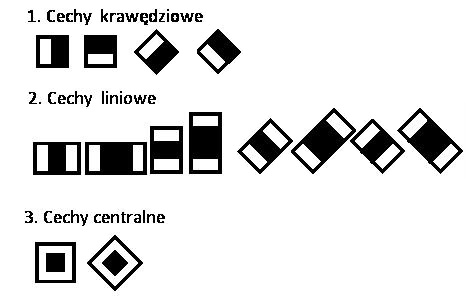
\includegraphics[scale=0.6]{./violajones.jpg}
\caption[Cechy rozpoznawane przez OpenCV]{Zestaw cech zaproponowany przez Lienhart'a i Maydt'a}
\end{figure}

Dla przykładu, prostokątne regiony oczu mają dużo mniejszą intensywnośd niż obszar czoła, ten zaś dużo większą od obszaru włosów 

\subsection{Tworzenie klasyfikatora kaskadowego}
Odbywa się z wykorzystaniem algorytmu uczącego \textbf{AdBoost}. Wykorzystuje on tzw. wzmocnienie adaptacyjne (ang. adaptive boosting). Jego
zadaniem jest wygenerowanie silnego klasyfikatoraz kaskady słabych. W przypadku obrazów, na których wykryty ma zostać obiekt wykorzystuje się technikę przesuwnego okna. Z tak zeskanowanego obrazu generowany jest zbiór okien, które poddawane są weryfikacji przez klasyfikatory. Na podstawie informacji z tych okien słabe klasyfikatory uczą się odrzucać obszary, na których na pewno nie znajduje się poszukiwany obiekt. W każdej pętli algorytm skupia się na źle wykrytych obszarach przez poprzednie klasyfikatory. Nadaje im wyższe wagi (gdyż w następnej iteracji istnieje większe prawdopodobieostwo prawidłowego wykrycia obiektu). Wykorzystywanie tych wag przez następne klasyfikatory pozwala na zawężenie przestrzeni poszukiwń do coraz mniejszego obszaru. Tak skonstruowany silny klasyfikator umożliwia szybkie wykrywanie poszukiwanych obiektów.


\section{Porównanie twarzy}
Twarze rozpoznane na zdjęciu zostają przekazane w celu ich porównania z twarzami dostępnymi w bazie. Porównywanie twarzy opiera się o szereg algorytmów.

\subsection{Kowariancja}
Kowariancja jest miarą tego, jak dalece wartości dwóch zmiennych losowych zmieniają się razem. Jeśli zmienne zachowują się podobnie, to kowariancja jest liczbą dodatnia, w przeciwnym razie kowariancja jest ujemna.
Macierz kowariancji to macierz której elementem na miejscu (i,j) jest kowariancja pomiędzy i-tym oraz j-tym elementem wektora losowego.   

\subsection{Analiza głównych składowych (PCA)}
Statystyczna metoda służąca odnajdywaniu struktur w zbiorze zmiennych losowych. Celem PCA jest przekształcenie zbioru obserwacji prawdopodobnie skorelowanych ze sobą zmiennych w zbiór wartości nieskorelowanych zmiennych zwanych głównymi składowymi. Transformacja ta jest zdefiniowana w taki sposób, że pierwsza główna składowa ma jak największą wariancję (czyli wyjaśnia tak  dużą część  zmienności danych jak to tylko możliwe), a każdy kolejny element ma jak największą wariancję pod warunkiem, że jest nie jest skorelowany z poprzednią składową.

\subsection{Eigenface}
Eigenface, lub twarze własne, to zbiór wektorów własnych używany przy komputerowym rozpoznaniu twarzy. Zbiór twarzy własnych może zostać wygenerowany przez wykonanie procedury PCA na dużym zbiorze obrazów ludzkich twarzy. Twarze własne można traktować jak zbiór "standaryzowanych składników twarzy". Każda ludzka twarz może być pojmowana jako kombinacja tych standardowych twarzy. Przykładowo czyjaś twarz może być kompozycją twarzy uśrednionej plus 10\% cech z twarzy własnej 1, 1,55\% z twarzy własnej nr 2 oraz nawet 3\% z twarzy własnej 3. 

\begin{figure}[h]
\centering
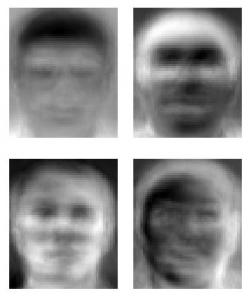
\includegraphics[scale=0.5]{./eigenface.jpg}
\caption[Twarze własne, przykłady]{Przykłady twarzy własnych z laboratorium AT\&T w Cambridge}
\end{figure}

Dzięki przechowywaniu twarzy nie jako pliku graficznego, a jako listy pewnych wartości, rozmiar pliku jest niewielki. Stworzone twarze własne będą ukazywać się jako jasne  ciemne obszary układające się w pewien określony zbiór.

\subsection{Algorytm k najbliższych sąsiadów}
Jest to algorytm uzywany w statystyce do prognozowania wartości pewnej zmiennej losowej, jednak może być również używany do klasyfikacji. Aby polepszyć działanie algorytmu kNN powszechnie stosowaną techniką jest \textbf{standaryzacja} lub \textbf{normalizacja} danych. Standaryzacja polega na doprowadzeniu do sytuacji w której wartość średnia poszczególnej cechy ma wartość 0 a odchylenie standardowe = 1. Normalizacja to  doprowadzenie do sytuacji w której wartości zmiennej należą do przedziału [0,1]
\newline \\
\textbf{Uczenie}:
\begin{enumerate}
  \item Dokonaj alternatywnie: standaryzacji/normalizacji/pozostaw dane jakie są
  \item Zapamiętaj cały zbiór treningowy
\end{enumerate}
\textbf{Testowanie}:
\begin{enumerate}
  \item Dokonaj standaryzacji/normalizacji/pozostaw dane jakie są (testowanie)
  \item Policz odległości pomiędzy wektorem testowym a wszystkimi wektorami zbioru treningowego
  \item Posortuj odległości od największej do najmniejszej
  \item Zobacz etykiety  k – najbliższych wektorów do wektora testowego.  Zrób histogram częstości poszczególnych etykiet spośród „k-najbliższych” (Policz ile i których etykiet było spośród k najbliższych)
  \item Przypisz najczęściej występującą etykietę jako etykietę wektora testowego 
  \item Jeśli wystąpił impas (dwie klasy miały taką samą liczbę głosów) rozwiąż problem losowo
\end{enumerate}
\pagebreak[4]


\section{Praktyczna realizacja zadania}

\begin{figure}[h]
\centering
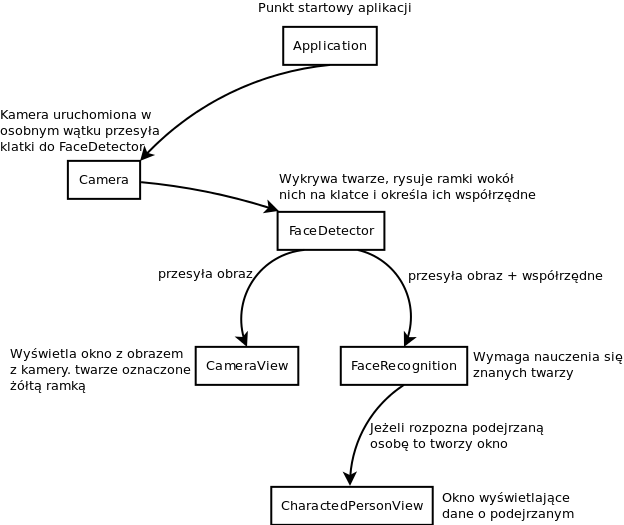
\includegraphics[scale=0.6]{./idea_dzialania_programu.png}
\caption[Idea działania programu]{Idea działania programu.}
\end{figure}

Obraz z kamery zostaje przekazany do klasy obserwatora, zostaje tam przetworzony, oraz następuje wychwycenie twarzy na zdjęciu. Interfejs graficzny otrzymuje przechwyconą klatkę z kamery, wraz z twarzami obramowanymi prostokątami i wyświetla obraz na ekranie. W tym samym czasie z klatki zostają wyodrębione wszystkie twarze, które są jednocześnie skalowane do rozmiaru 100\begin{math}\times\end{math}100 pikseli, a ich barwy są zmieniane do skali szarości. Dzięki wykorzystaniu wzorca projektowego obserwator, przy każdej zmianie obrazu na kamerze klasa otrzymuje nowy obraz, a natychmiast po przetworzeniu obrazu klasy nasłuchujące otrzymują wymagane dane (klatka z obramowaniem, wycięte twarze). 


\pagebreak[4]


\section{Wnioski i uwagi}



\listoffigures


\end{document}
